%! suppress = MissingImport
If your momentary pushbuttons are attached to a cardboard strip with tape, remove them from the cardboard strip.
If your momentary pushbuttons' leads have metal tabs at the end (Figure~\ref{fig:pushbutton-tabs}), you will need to snip off the tabs before inserting the pushbutton leads into the breadboard;
ordinary scissors will suffice for this task.
Regardless of whether the leads have metal tabs at the end, you may optionally trim the leads to be about $\frac{1}{4}$in (6.4mm) long -- you can use the exposed lead from a jumper wire as a reference -- so that the pushbuttons sit flush on the breadboard.
It is not necessary that they sit flush;
this is simply to keep the buttons from wiggling under your fingers.
\textit{Do not cut the leads shorter than $\mathit{\frac{1}{8}}$in (3.2mm)!}
\textbf{Be sure to use eye protection in case the leads' ends fly off when you snip them.}

These are ``normally open'' momentary ``switches'' that close when pressed and re-open when released.
We will wire the pushbuttons such that they normally produce a 1, and when pressed will produce a 0.
Figure~\ref{fig:pushbutton-diagram} shows a diagram of the wiring for the pushbuttons.

\begin{figure}
    \centering
    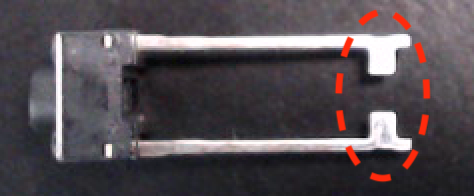
\includegraphics[height=2cm]{direct/buttons/pushbutton-tabs}
    \caption{Some momentary pushbuttons have metal tabs on their leads.\label{fig:pushbutton-tabs}}
\end{figure}

\begin{figure}
    \centering
    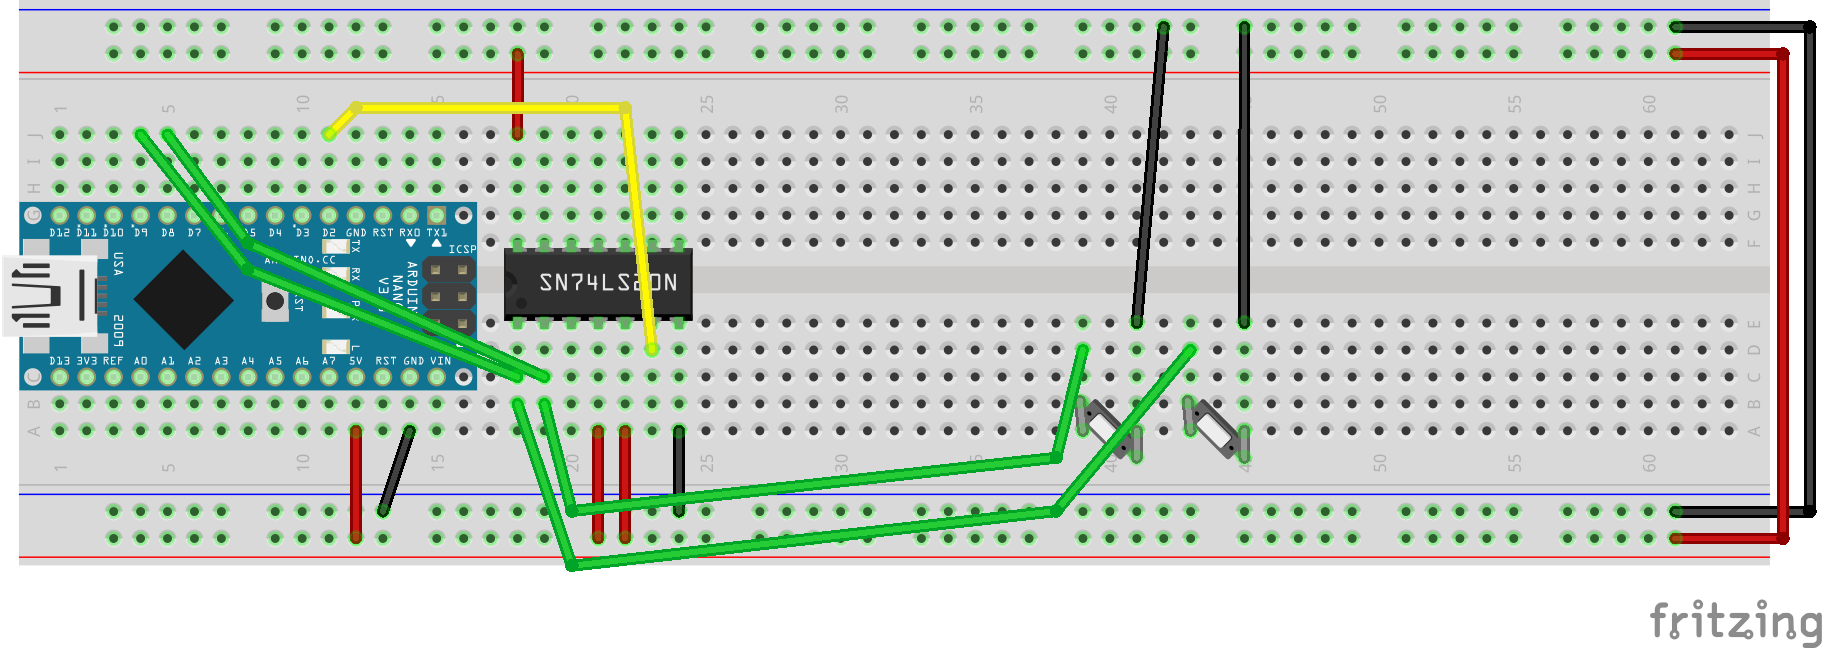
\includegraphics[width=0.9\textwidth]{fritzing_diagrams/pushbutton}
    \caption{Diagram of wiring associated with momentary pushbutton input.
        \textit{Note: connection between the 74LS20's pin 6 and the \developmentboard's
        \texttt{D2} pin was previously installed in Section~\ref{subsec:nand}.}
        \label{fig:pushbutton-diagram}}
\end{figure}

\disconnect\

Insert the leads of one pushbutton into contact points a39 and a41.
Peel off one wire from the \rainbow, and use it to connect contact point e41 to the upper \ground.
Insert the leads of the other pushbutton into contact points a43 and a45.
Peel off one wire from the \rainbow, and use it to connect contact point e45 to the upper \ground.
See Figure~\ref{fig:pushbutton-grounded}.

Peel off a 2-conductor cable from the \rainbow, and use it to connect contact points a21 and a22 (electrically connected to the 74LS20's \texttt{C1} and \texttt{D1}, pins 4 and 5) to a \power.
Peel off another 2-conductor cable and use it to connect contact points d39 and d43 (electrically connected to the ungrounded sides of the pushbuttons) to the 74LS20: contact point d39 should be connected to contact point b19 (electrically connected to the 74LS20's \texttt{B1}, pin 2), and contact point d43 should be connected to contact point b18 (electrically connected to the 74LS20's \texttt{A1}, pin 1).
See Figure~\ref{fig:pushbutton-nand}.

Peel off another 2-conductor cable from the \rainbow, and use it to connect contact points j4 and j5 (electrically connected to the \developmentboard's \texttt{D9} and \texttt{D8} pins) to contact points c18 and c19 (electrically connected to the 74LS20's \texttt{A1} and \texttt{B1}, and to the pushbuttons through the cable you installed in the previous paragraph), respectively.
See Figure~\ref{fig:pushbutton-nano}.

\begin{figure}\begin{multicols}{2}
    \centering
    \subfloat[The momentary pushbuttons, each with one lead grounded.]{
        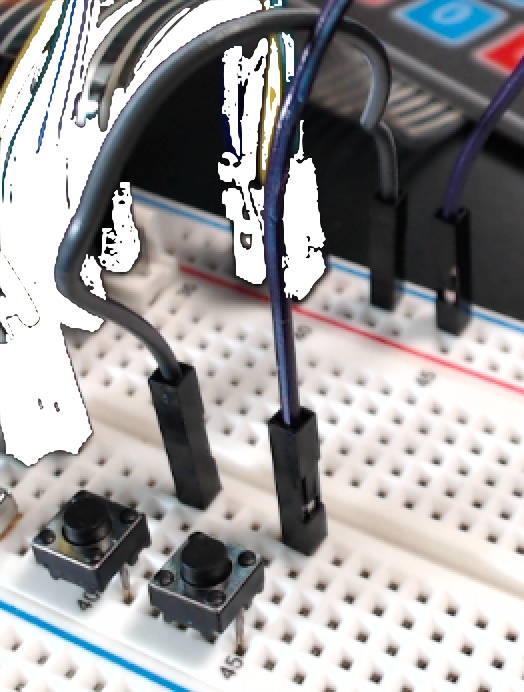
\includegraphics[width=0.4\textwidth]{direct/buttons/pushbutton-grounded}
        \label{fig:pushbutton-grounded}
    }
    \columnbreak

    \subfloat[Connections between the momentary pushbuttons and the 74LS20.]{
        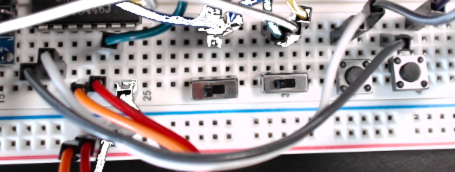
\includegraphics[width=0.55\textwidth]{direct/buttons/pushbutton-nand}
        \label{fig:pushbutton-nand}
    }

    \subfloat[Connections between the \developmentboard\ and wiring to the momentary
        pushbuttons.]{
        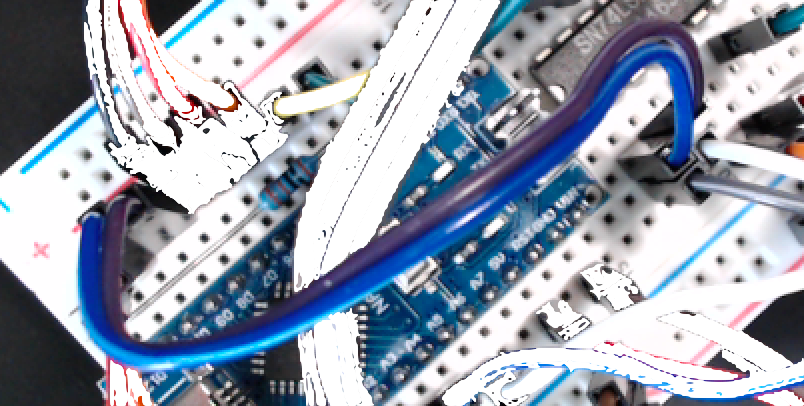
\includegraphics[width=.55\textwidth]{direct/buttons/pushbutton-nano}
        \label{fig:pushbutton-nano}
    }
    \end{multicols}
    \caption{Wiring the Momentary Pushbuttons.}
\end{figure}

When you have finished setting up the pushbuttons' wiring, there should be the electrical paths described in Table~\ref{tab:pushbutton}.

\begin{table}
    \begin{center}\begin{tabular}{||c|c|c|c||} \hline\hline
    Pushbutton                      & 74LS20            & \developmentboard\ pin    & Pulled High/Low \\ \hline
    Left button's grounded lead     &                   &               & Pulled Low \\
    Left button's ungrounded lead   & Lower NAND Input  & \texttt{D8}   & \\
    Right button's grounded lead    &                   &               & Pulled Low \\
    Right button's ungrounded lead  & Lower NAND Input  & \texttt{D9}   & \\
                                    & Lower NAND Input  &               & Pulled High \\
                                    & Lower NAND Input  &               & Pulled High \\
                                    & Lower NAND Output & \texttt{D2}   & \\ \hline\hline
    \end{tabular}\end{center}
    \caption{Electrical Paths for Momentary Pushbuttons.\label{tab:pushbutton}}
\end{table}

\checkpoint{inserted and wired the momentary pushbuttons}

Connect your \developmentboard\ to the computer.
In the IDE's Serial Monitor, notice that the LEFT~BUTTON is always 1, the RIGHT~BUTTON is always 1, and the BUTTON~NAND is always 0.
Notice that when you press a button, the Serial Monitor shows that its value becomes 0, and when you release a button, its value becomes 1 again.
If either button is pressed, BUTTON~NAND becomes 1, and it is 0 only when both buttons are not pressed.